% !TEX root = ../master.tex

\vspace*{.5cm}
\section{Universitäts- und Landesbibliothek Münster}
\begin{center}
\emph{Viola Voß}
\end{center}
\vspace*{1cm}

%body
\hypertarget{zeigen-sie-uns-den-ort-in-ihrer-bibliothek-an-dem-sie-die-meiste-zeit-verbringen.-was-ist-das-fuxfcr-ein-ort-wieso-sind-sie-die-meiste-zeit-dort}{%
\subsubsection*{Zeigen Sie uns den Ort in Ihrer Bibliothek, an dem Sie die
meiste Zeit verbringen. Was ist das für ein Ort? Wieso sind Sie die
meiste Zeit
dort?}\label{zeigen-sie-uns-den-ort-in-ihrer-bibliothek-an-dem-sie-die-meiste-zeit-verbringen.-was-ist-das-fuxfcr-ein-ort-wieso-sind-sie-die-meiste-zeit-dort}}

\begin{center}
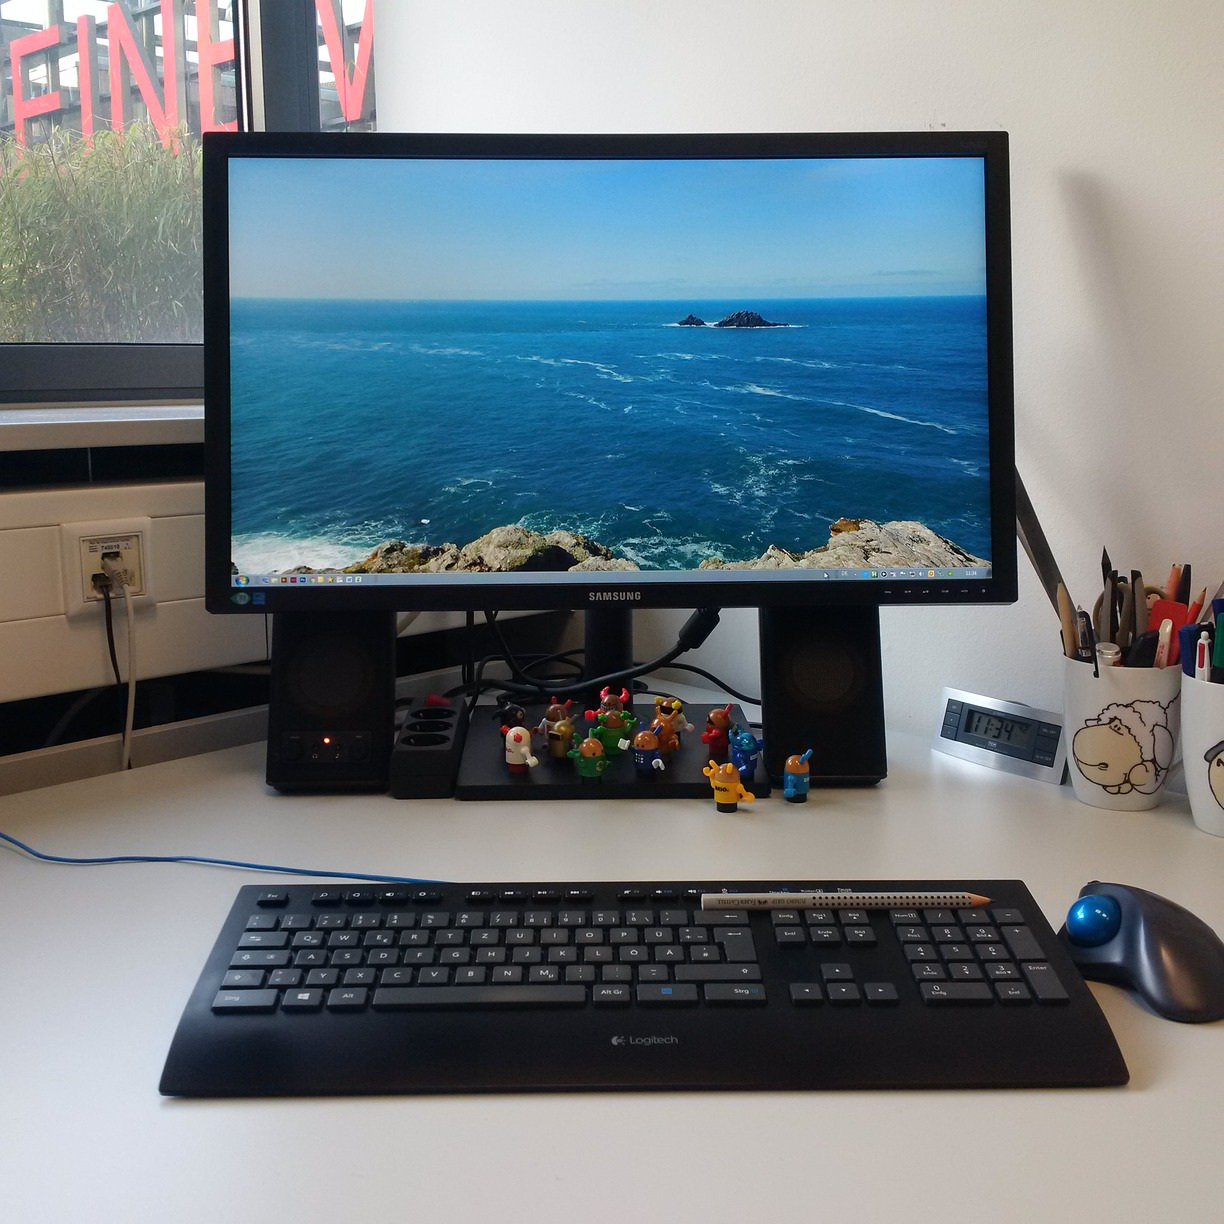
\includegraphics[width=0.5\textwidth]{ulb-muenster/img/schreibtisch.jpg}
\end{center}

Mein Schreibtisch in meinem Büro.

Ich bin zwischendurch auch in einigen unserer dezentralen Bibliotheken
unterwegs, aber die meiste Zeit sitze ich hier im Zentralgebäude.

\hypertarget{was-wuxfcrden-sie-vermissen-wenn-es-nicht-mehr-da-wuxe4re-wieso-wuxfcrden-sie-es-vermissen}{%
\subsubsection*{Was würden Sie vermissen, wenn es nicht mehr da wäre? Wieso
würden Sie es
vermissen?}\label{was-wuxfcrden-sie-vermissen-wenn-es-nicht-mehr-da-wuxe4re-wieso-wuxfcrden-sie-es-vermissen}}

\begin{center}
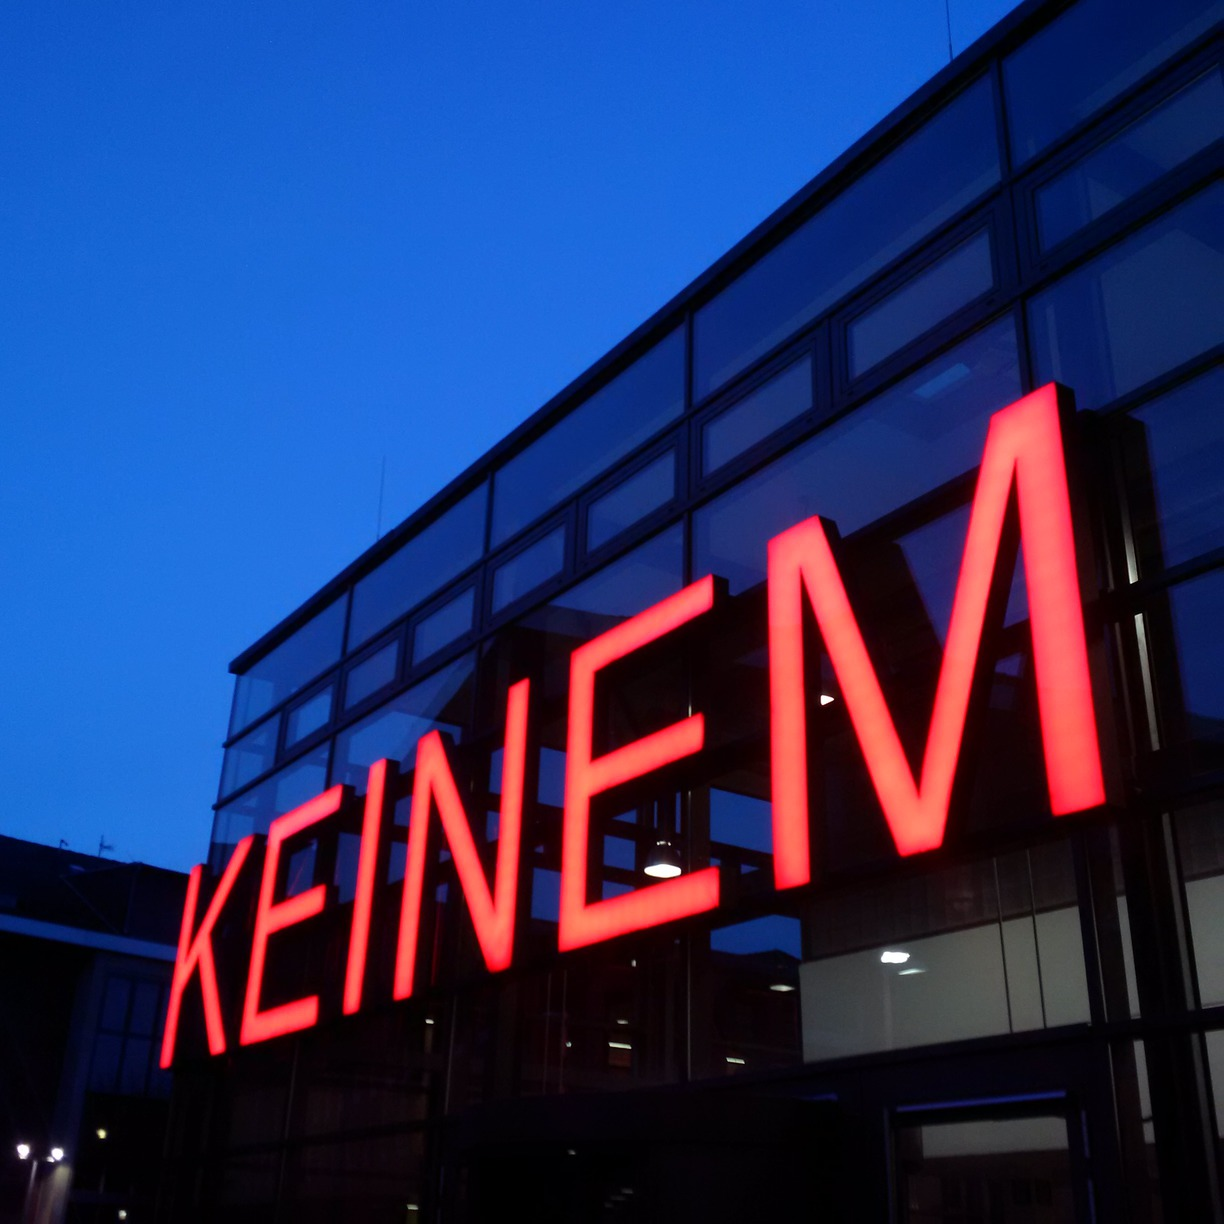
\includegraphics[width=0.5\textwidth]{ulb-muenster/img/schriftzug.jpg}
\end{center}

Unseren Kunst-am-Bau-Schriftzug \enquote{Gehorche Keinem}.

Kunst, die speziell für diesen Ort geschaffen wurde, die zum Denken
anregt und die dabei auch noch gut aussieht.\footnote{\href{https://www.ulb.uni-muenster.de/bibliothek/profil/gehorchekeinem.html}{https://www.ulb.uni-muenster.de/bibliothek/profil/gehorchekeinem.html}}

\hypertarget{was-stuxf6rt-sie-an-ihrer-bibliothek-beziehungsweise-was-wuxfcrden-sie-gerne-verbessern-wieso-stuxf6rt-sie-das-jetzt-noch}{%
\subsubsection*{Was stört Sie an Ihrer Bibliothek beziehungsweise was würden
Sie gerne verbessern? Wieso stört Sie das jetzt
(noch)?}\label{was-stuxf6rt-sie-an-ihrer-bibliothek-beziehungsweise-was-wuxfcrden-sie-gerne-verbessern-wieso-stuxf6rt-sie-das-jetzt-noch}}

\begin{center}
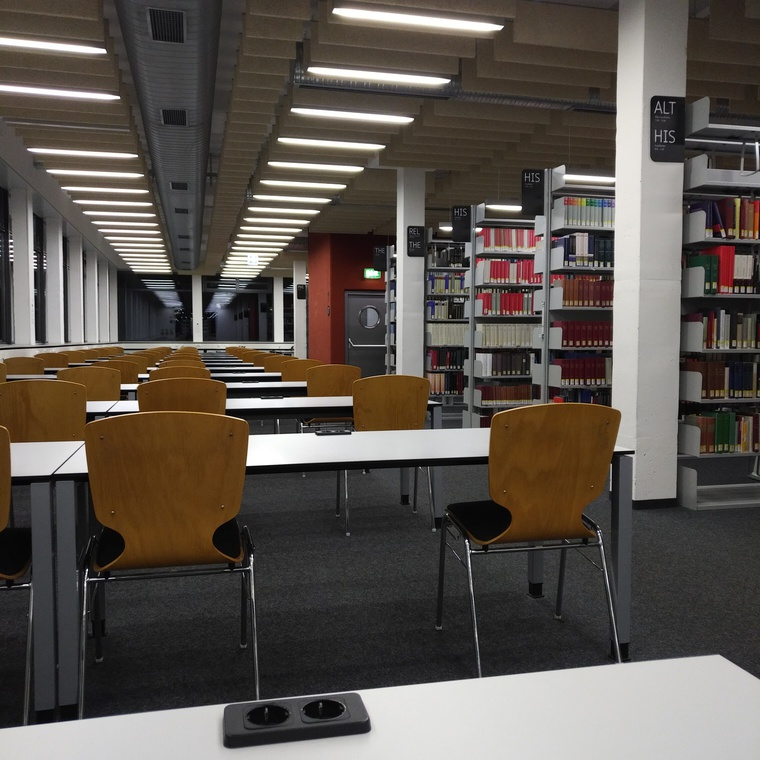
\includegraphics[width=0.5\textwidth]{ulb-muenster/img/arbeitsplaetze.jpg}
\end{center}

Wir haben schon viele Arbeitsplätze -- aber es müssten noch sehr viel
mehr sein. Vor allem Gruppenarbeitsplätze. Wie in jeder Bibliothek.

Dabei oft gegeneinander abzuwägen: Arbeitsplätze versus
(Freihand-)Bestand.

Es gibt bereits Pläne für eine Erweiterung unserer Gruppenarbeitsplätze,
aber die Umsetzung wird baubedingt noch einige Zeit dauern.

\hypertarget{zeigen-sie-uns-spuren-der-bibliotheksnutzung.-gibt-es-dazu-eine-geschichte}{%
\subsubsection*{Zeigen Sie uns Spuren der Bibliotheksnutzung. Gibt es dazu eine
Geschichte?}\label{zeigen-sie-uns-spuren-der-bibliotheksnutzung.-gibt-es-dazu-eine-geschichte}}

\begin{center}
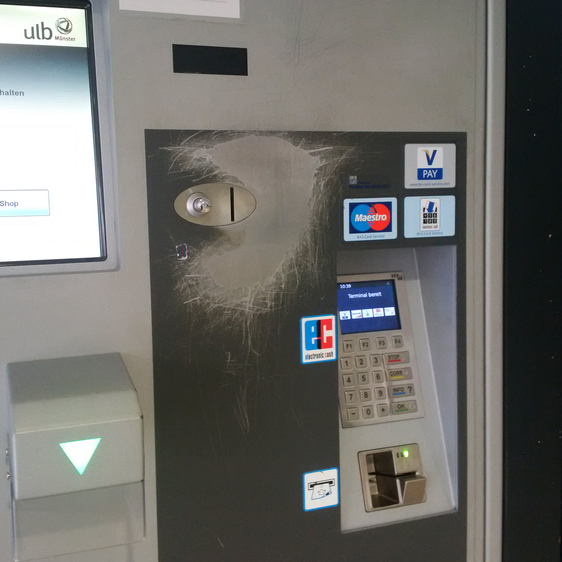
\includegraphics[width=0.5\textwidth]{ulb-muenster/img/kassenautomat.jpg}
\end{center}

Unser Kassenautomat.

Es gibt offenbar immer noch viele Leute, die meinen, dass das Rubbeln
von Münzen die Akzeptanzquote von Automaten erhöht.

\hypertarget{was-haben-sie-was-die-anderen-nicht-haben-warum-haben-sie-das-sollten-andere-es-auch-in-ihren-bibliotheken-haben}{%
\subsubsection*{Was haben Sie, was die anderen nicht haben? Warum haben Sie
das? Sollten andere es auch in ihren Bibliotheken
haben?}\label{was-haben-sie-was-die-anderen-nicht-haben-warum-haben-sie-das-sollten-andere-es-auch-in-ihren-bibliotheken-haben}}

\begin{center}
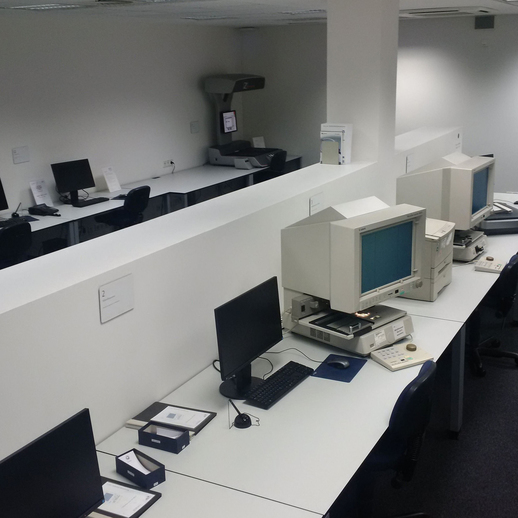
\includegraphics[width=0.5\textwidth]{ulb-muenster/img/DigiLab.jpg}
\end{center}

Unser DigiLab: Scanner von A4 bis A2 und für Mikromaterialien sowie
Rechner mit DTP- und Textverarbeitungs-Software zur kostenlosen Nutzung
für alle Benutzer.\footnote{\href{https://www.ulb.uni-muenster.de/digilab}{https://www.ulb.uni-muenster.de/digilab}}

\hypertarget{ihre-bibliothek-name-adresse-spezialisierung-was-man-noch-uxfcber-sie-wissen-sollte}{%
\subsubsection*{Ihre Bibliothek (Name, Adresse, Spezialisierung, was man noch
über sie wissen
sollte)?}\label{ihre-bibliothek-name-adresse-spezialisierung-was-man-noch-uxfcber-sie-wissen-sollte}}

Universitäts- und Landesbibliothek Münster\footnote{\href{https://www.ulb.uni-muenster.de/}{https://www.ulb.uni-muenster.de/}}

Krummer Timpen 3, 48143 Münster

%autor
\begin{center}\rule{0.5\linewidth}{\linethickness}\end{center}

\textbf{Viola Voß}, Fachreferentin für die Fächer und die Bibliotheken
im Fachbereich 9 (Philologie) der Westfälischen Wilhelms-Universität
Münster, interessiert an Embedded Librarianship, Bibliotheksmanagement,
Wissensmanagement sowie Open Access und Open Science.
Sprachwissenschaftlerin. ORCID:
\href{https://orcid.org/0000-0003-3056-407X}{https://orcid.org/0000-0003-3056-407X}